\documentclass[11pt,]{article}
\usepackage[left=1in,top=1in,right=1in,bottom=1in]{geometry}
\newcommand*{\authorfont}{\fontfamily{phv}\selectfont}
\usepackage[]{mathpazo}


  \usepackage[T1]{fontenc}
  \usepackage[utf8]{inputenc}



\usepackage{abstract}
\renewcommand{\abstractname}{}    % clear the title
\renewcommand{\absnamepos}{empty} % originally center

\renewenvironment{abstract}
 {{%
    \setlength{\leftmargin}{0mm}
    \setlength{\rightmargin}{\leftmargin}%
  }%
  \relax}
 {\endlist}

\makeatletter
\def\@maketitle{%
  \newpage
%  \null
%  \vskip 2em%
%  \begin{center}%
  \let \footnote \thanks
    {\fontsize{18}{20}\selectfont\raggedright  \setlength{\parindent}{0pt} \@title \par}%
}
%\fi
\makeatother




\setcounter{secnumdepth}{3}

\usepackage{color}
\usepackage{fancyvrb}
\newcommand{\VerbBar}{|}
\newcommand{\VERB}{\Verb[commandchars=\\\{\}]}
\DefineVerbatimEnvironment{Highlighting}{Verbatim}{commandchars=\\\{\}}
% Add ',fontsize=\small' for more characters per line
\usepackage{framed}
\definecolor{shadecolor}{RGB}{248,248,248}
\newenvironment{Shaded}{\begin{snugshade}}{\end{snugshade}}
\newcommand{\KeywordTok}[1]{\textcolor[rgb]{0.13,0.29,0.53}{\textbf{#1}}}
\newcommand{\DataTypeTok}[1]{\textcolor[rgb]{0.13,0.29,0.53}{#1}}
\newcommand{\DecValTok}[1]{\textcolor[rgb]{0.00,0.00,0.81}{#1}}
\newcommand{\BaseNTok}[1]{\textcolor[rgb]{0.00,0.00,0.81}{#1}}
\newcommand{\FloatTok}[1]{\textcolor[rgb]{0.00,0.00,0.81}{#1}}
\newcommand{\ConstantTok}[1]{\textcolor[rgb]{0.00,0.00,0.00}{#1}}
\newcommand{\CharTok}[1]{\textcolor[rgb]{0.31,0.60,0.02}{#1}}
\newcommand{\SpecialCharTok}[1]{\textcolor[rgb]{0.00,0.00,0.00}{#1}}
\newcommand{\StringTok}[1]{\textcolor[rgb]{0.31,0.60,0.02}{#1}}
\newcommand{\VerbatimStringTok}[1]{\textcolor[rgb]{0.31,0.60,0.02}{#1}}
\newcommand{\SpecialStringTok}[1]{\textcolor[rgb]{0.31,0.60,0.02}{#1}}
\newcommand{\ImportTok}[1]{#1}
\newcommand{\CommentTok}[1]{\textcolor[rgb]{0.56,0.35,0.01}{\textit{#1}}}
\newcommand{\DocumentationTok}[1]{\textcolor[rgb]{0.56,0.35,0.01}{\textbf{\textit{#1}}}}
\newcommand{\AnnotationTok}[1]{\textcolor[rgb]{0.56,0.35,0.01}{\textbf{\textit{#1}}}}
\newcommand{\CommentVarTok}[1]{\textcolor[rgb]{0.56,0.35,0.01}{\textbf{\textit{#1}}}}
\newcommand{\OtherTok}[1]{\textcolor[rgb]{0.56,0.35,0.01}{#1}}
\newcommand{\FunctionTok}[1]{\textcolor[rgb]{0.00,0.00,0.00}{#1}}
\newcommand{\VariableTok}[1]{\textcolor[rgb]{0.00,0.00,0.00}{#1}}
\newcommand{\ControlFlowTok}[1]{\textcolor[rgb]{0.13,0.29,0.53}{\textbf{#1}}}
\newcommand{\OperatorTok}[1]{\textcolor[rgb]{0.81,0.36,0.00}{\textbf{#1}}}
\newcommand{\BuiltInTok}[1]{#1}
\newcommand{\ExtensionTok}[1]{#1}
\newcommand{\PreprocessorTok}[1]{\textcolor[rgb]{0.56,0.35,0.01}{\textit{#1}}}
\newcommand{\AttributeTok}[1]{\textcolor[rgb]{0.77,0.63,0.00}{#1}}
\newcommand{\RegionMarkerTok}[1]{#1}
\newcommand{\InformationTok}[1]{\textcolor[rgb]{0.56,0.35,0.01}{\textbf{\textit{#1}}}}
\newcommand{\WarningTok}[1]{\textcolor[rgb]{0.56,0.35,0.01}{\textbf{\textit{#1}}}}
\newcommand{\AlertTok}[1]{\textcolor[rgb]{0.94,0.16,0.16}{#1}}
\newcommand{\ErrorTok}[1]{\textcolor[rgb]{0.64,0.00,0.00}{\textbf{#1}}}
\newcommand{\NormalTok}[1]{#1}
\usepackage{longtable,booktabs}

\usepackage{graphicx,grffile}
\makeatletter
\def\maxwidth{\ifdim\Gin@nat@width>\linewidth\linewidth\else\Gin@nat@width\fi}
\def\maxheight{\ifdim\Gin@nat@height>\textheight\textheight\else\Gin@nat@height\fi}
\makeatother
% Scale images if necessary, so that they will not overflow the page
% margins by default, and it is still possible to overwrite the defaults
% using explicit options in \includegraphics[width, height, ...]{}
\setkeys{Gin}{width=\maxwidth,height=\maxheight,keepaspectratio}

\title{Patrones de las hormigas en el campus de la UASD, según el lugar donde
se recolectan.\\
Identificación y distribución.  }



\author{\Large Emma M. Diloné Ricardo\vspace{0.05in} \newline\normalsize\emph{Estudiante, Universidad Autónoma de Santo Domingo (UASD)}  }


\date{}

\usepackage{titlesec}

\titleformat*{\section}{\normalsize\bfseries}
\titleformat*{\subsection}{\normalsize\itshape}
\titleformat*{\subsubsection}{\normalsize\itshape}
\titleformat*{\paragraph}{\normalsize\itshape}
\titleformat*{\subparagraph}{\normalsize\itshape}

\titlespacing{\section}
{0pt}{36pt}{0pt}
\titlespacing{\subsection}
{0pt}{36pt}{0pt}
\titlespacing{\subsubsection}
{0pt}{36pt}{0pt}





\newtheorem{hypothesis}{Hypothesis}
\usepackage{setspace}

\makeatletter
\@ifpackageloaded{hyperref}{}{%
\ifxetex
  \PassOptionsToPackage{hyphens}{url}\usepackage[setpagesize=false, % page size defined by xetex
              unicode=false, % unicode breaks when used with xetex
              xetex]{hyperref}
\else
  \PassOptionsToPackage{hyphens}{url}\usepackage[unicode=true]{hyperref}
\fi
}

\@ifpackageloaded{color}{
    \PassOptionsToPackage{usenames,dvipsnames}{color}
}{%
    \usepackage[usenames,dvipsnames]{color}
}
\makeatother
\hypersetup{breaklinks=true,
            bookmarks=true,
            pdfauthor={Emma M. Diloné Ricardo (Estudiante, Universidad Autónoma de Santo Domingo (UASD))},
             pdfkeywords = {Hormigas, Campus UASD, suelo, dosel, género.},  
            pdftitle={Patrones de las hormigas en el campus de la UASD, según el lugar donde
se recolectan.\\
Identificación y distribución.},
            colorlinks=true,
            citecolor=blue,
            urlcolor=blue,
            linkcolor=magenta,
            pdfborder={0 0 0}}
\urlstyle{same}  % don't use monospace font for urls

% set default figure placement to htbp
\makeatletter
\def\fps@figure{htbp}
\makeatother

\usepackage{pdflscape} \newcommand{\blandscape}{\begin{landscape}}
\newcommand{\elandscape}{\end{landscape}}


% add tightlist ----------
\providecommand{\tightlist}{%
\setlength{\itemsep}{0pt}\setlength{\parskip}{0pt}}

\begin{document}
	
% \pagenumbering{arabic}% resets `page` counter to 1 
%
% \maketitle

{% \usefont{T1}{pnc}{m}{n}
\setlength{\parindent}{0pt}
\thispagestyle{plain}
{\fontsize{18}{20}\selectfont\raggedright 
\maketitle  % title \par  

}

{
   \vskip 13.5pt\relax \normalsize\fontsize{11}{12} 
\textbf{\authorfont Emma M. Diloné Ricardo} \hskip 15pt \emph{\small Estudiante, Universidad Autónoma de Santo Domingo (UASD)}   

}

}








\begin{abstract}

    \hbox{\vrule height .2pt width 39.14pc}

    \vskip 8.5pt % \small 

\noindent Los géneros de hormigas que se identifican en el campus de la UASD
pueden obedecer a diferentes patrones, lo que se busca establecer es si
uno de esos patrones tiene que ver con el lugar en el cual fueron
recolectadas. Para dar respuesta a esta incertidumbre, se realiza un
análisis por medio de un dendrograma, el cual agrupa las muestras
recolectadas por similitud entre ellas.


\vskip 8.5pt \noindent \emph{Keywords}: Hormigas, Campus UASD, suelo, dosel, género. \par

    \hbox{\vrule height .2pt width 39.14pc}



\end{abstract}


\vskip 6.5pt


\noindent  \begin{center}\rule{0.5\linewidth}{\linethickness}\end{center}

\begin{figure}
\centering
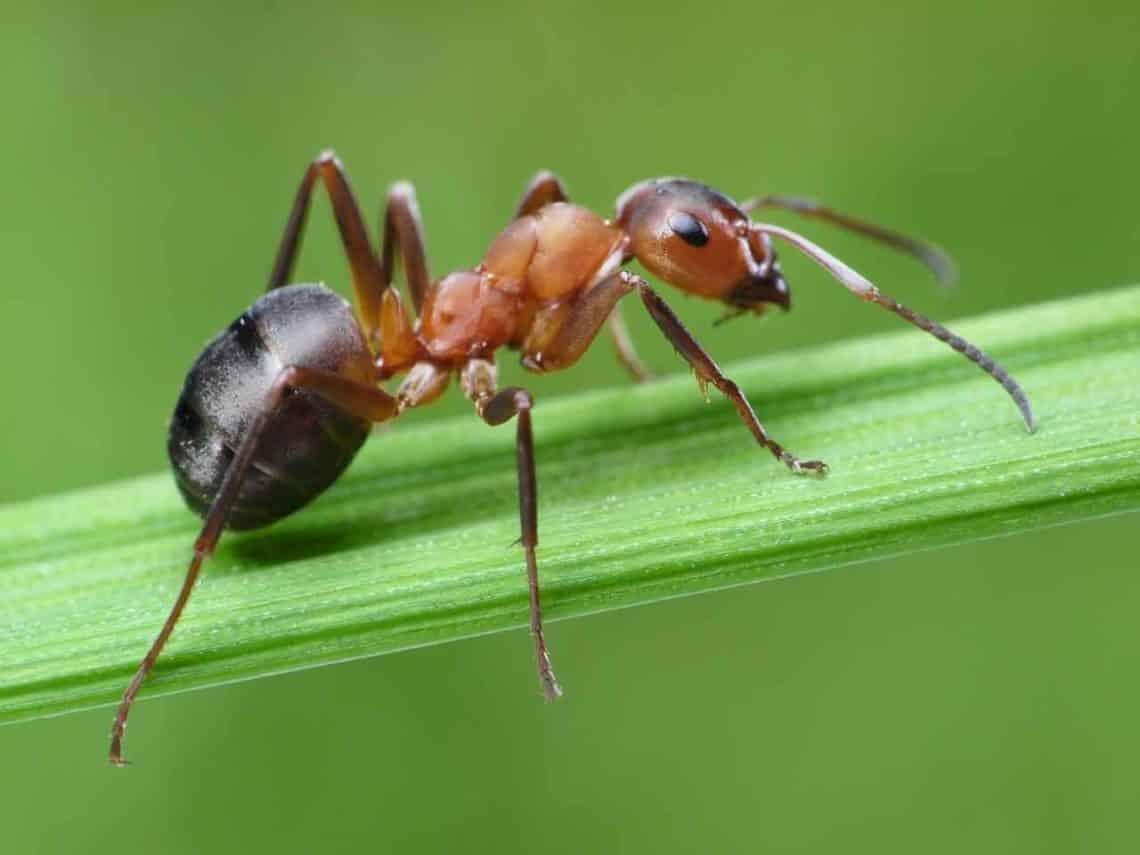
\includegraphics{Hormiga-1.jpg}
\caption{}
\end{figure}

\section{Introducción}\label{introducciuxf3n}

La Republica Dominicana está localizada en la isla La Hispaniola, en la
región del Caribe (figure 2), formando parte del arco de las denominadas
Antillas Mayores. Ocupa las dos terceras partes del este de la isla, la
cual comparte con la República de Haíti (figure 3). El campus de la
Universidad Autónoma de Santo Domingo (UASD) se encuentra en la ciudad
de Santo Domingo, República Dominicana.

\begin{figure}
\centering
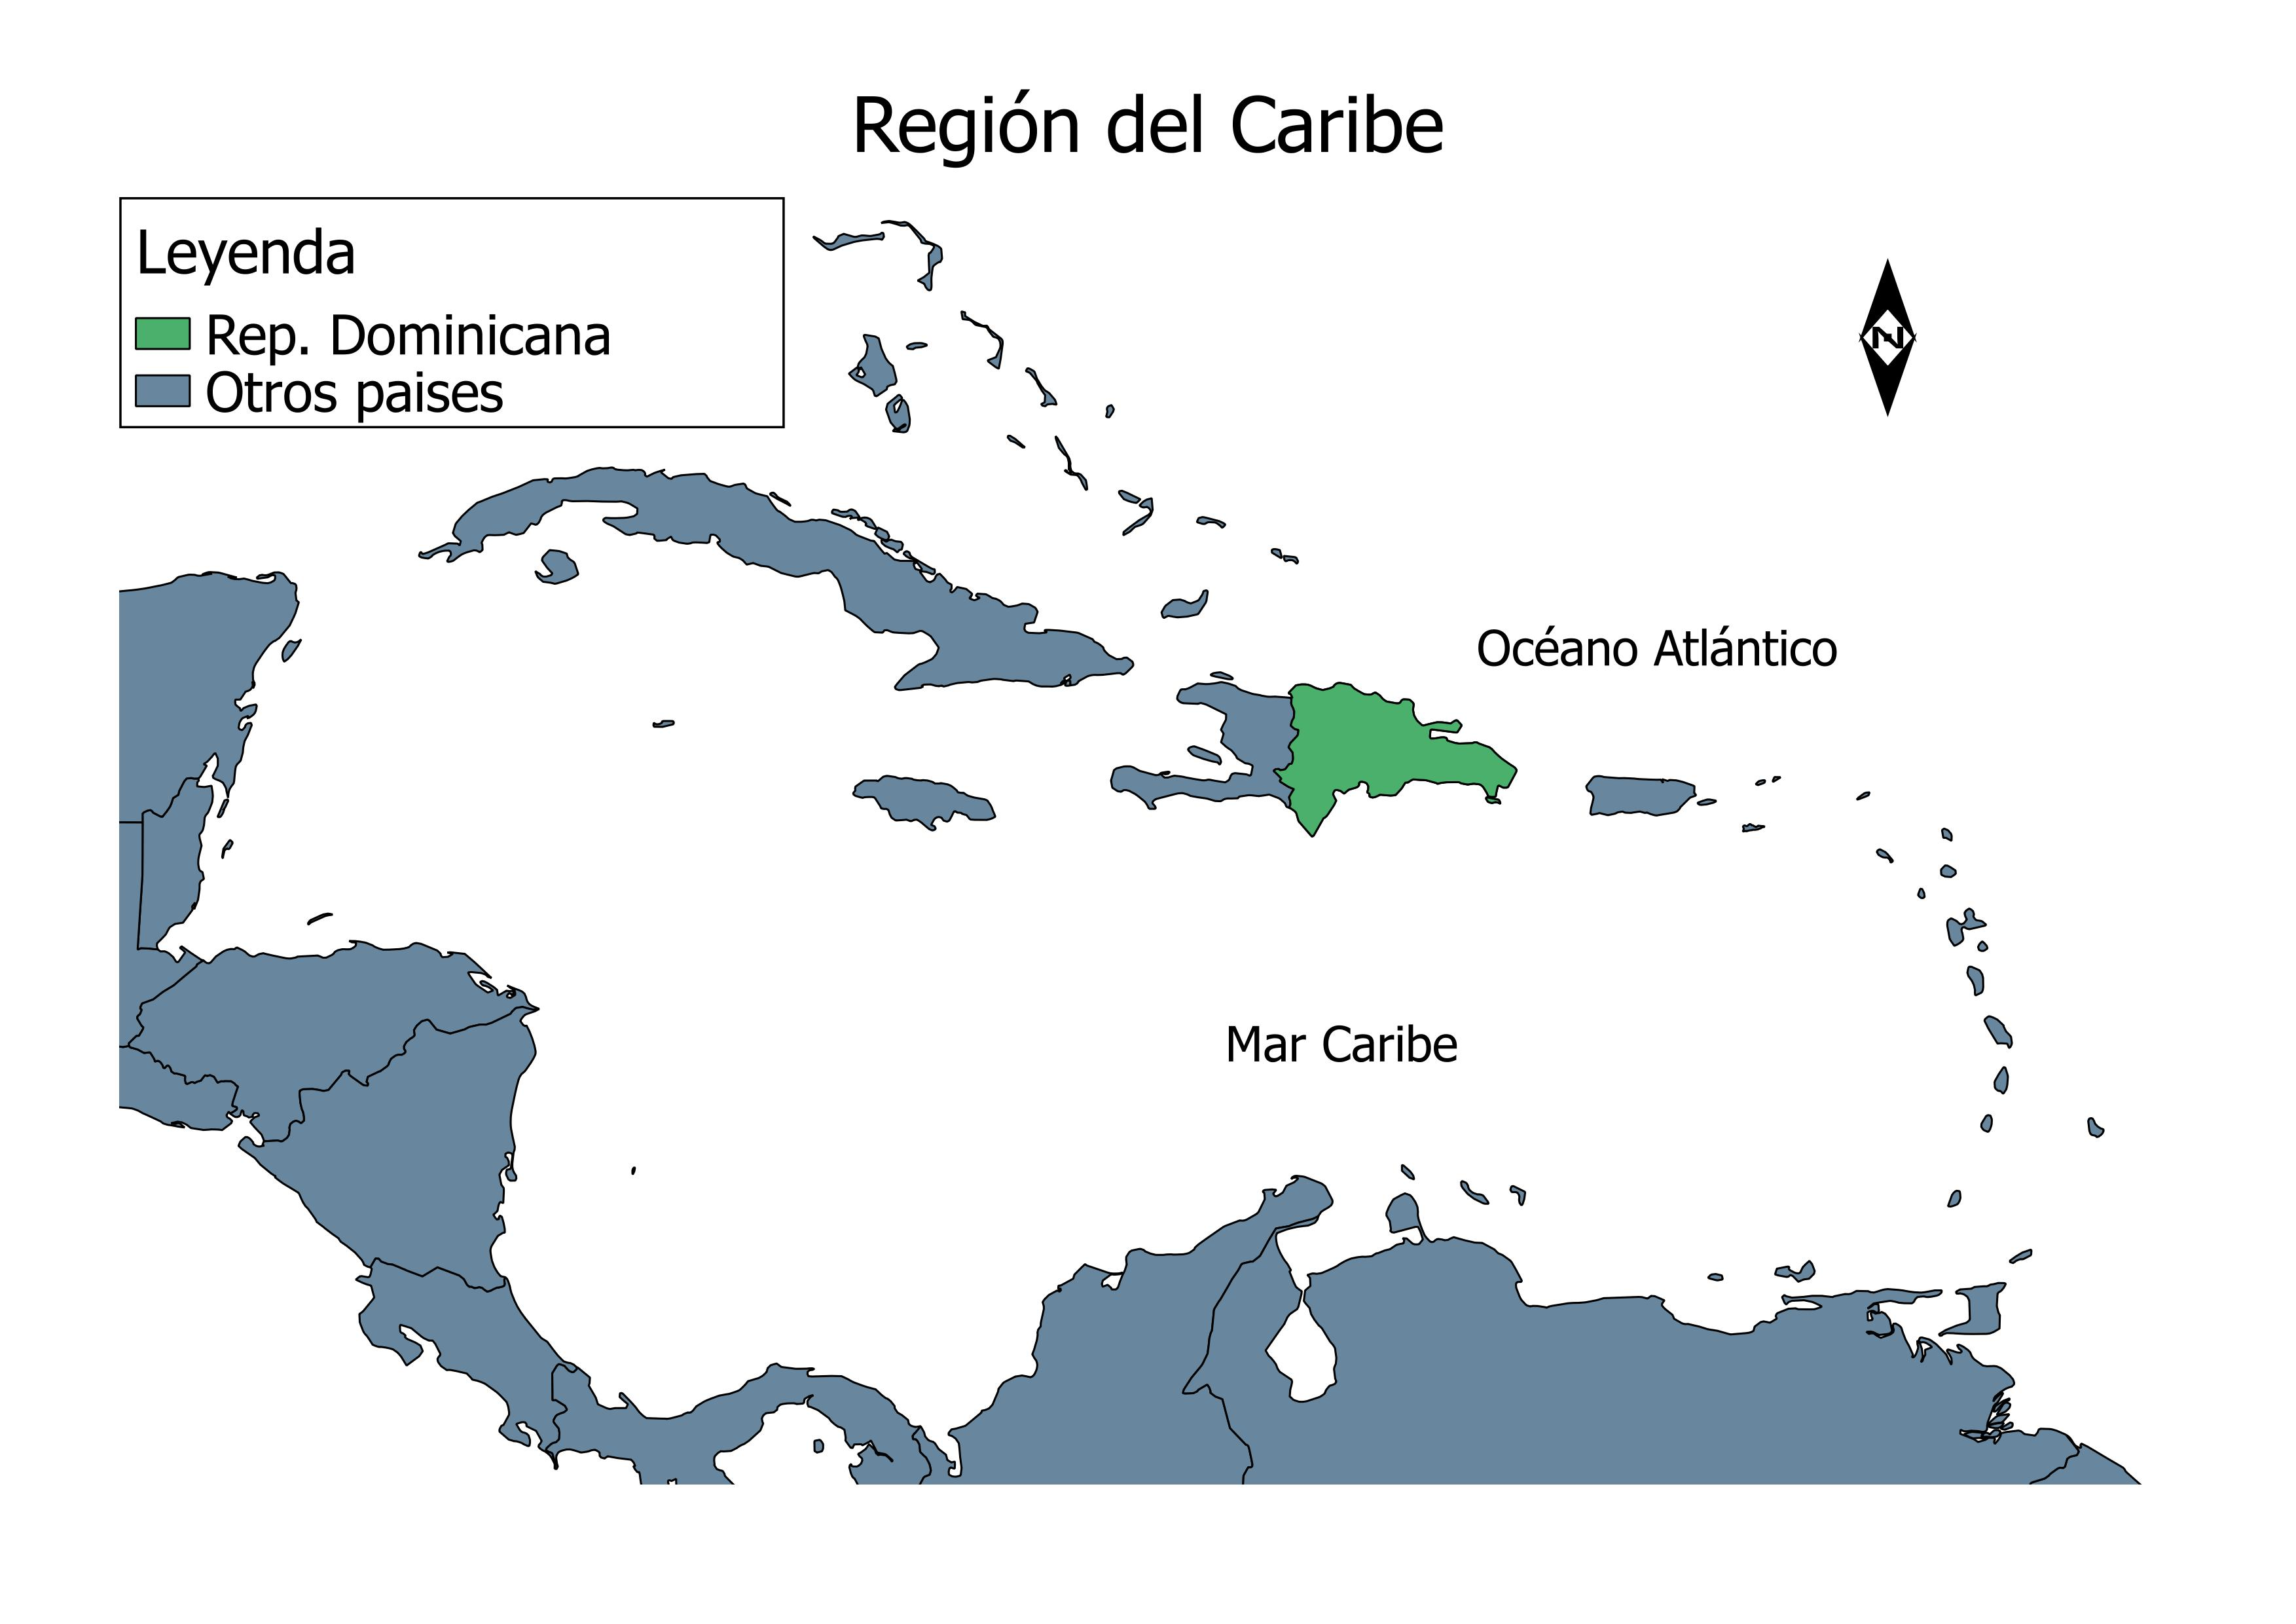
\includegraphics{caribe.jpeg}
\caption{Localización de la Rep.~Dominicana dentro de la región del
Caribe}
\end{figure}

\begin{figure}
\centering
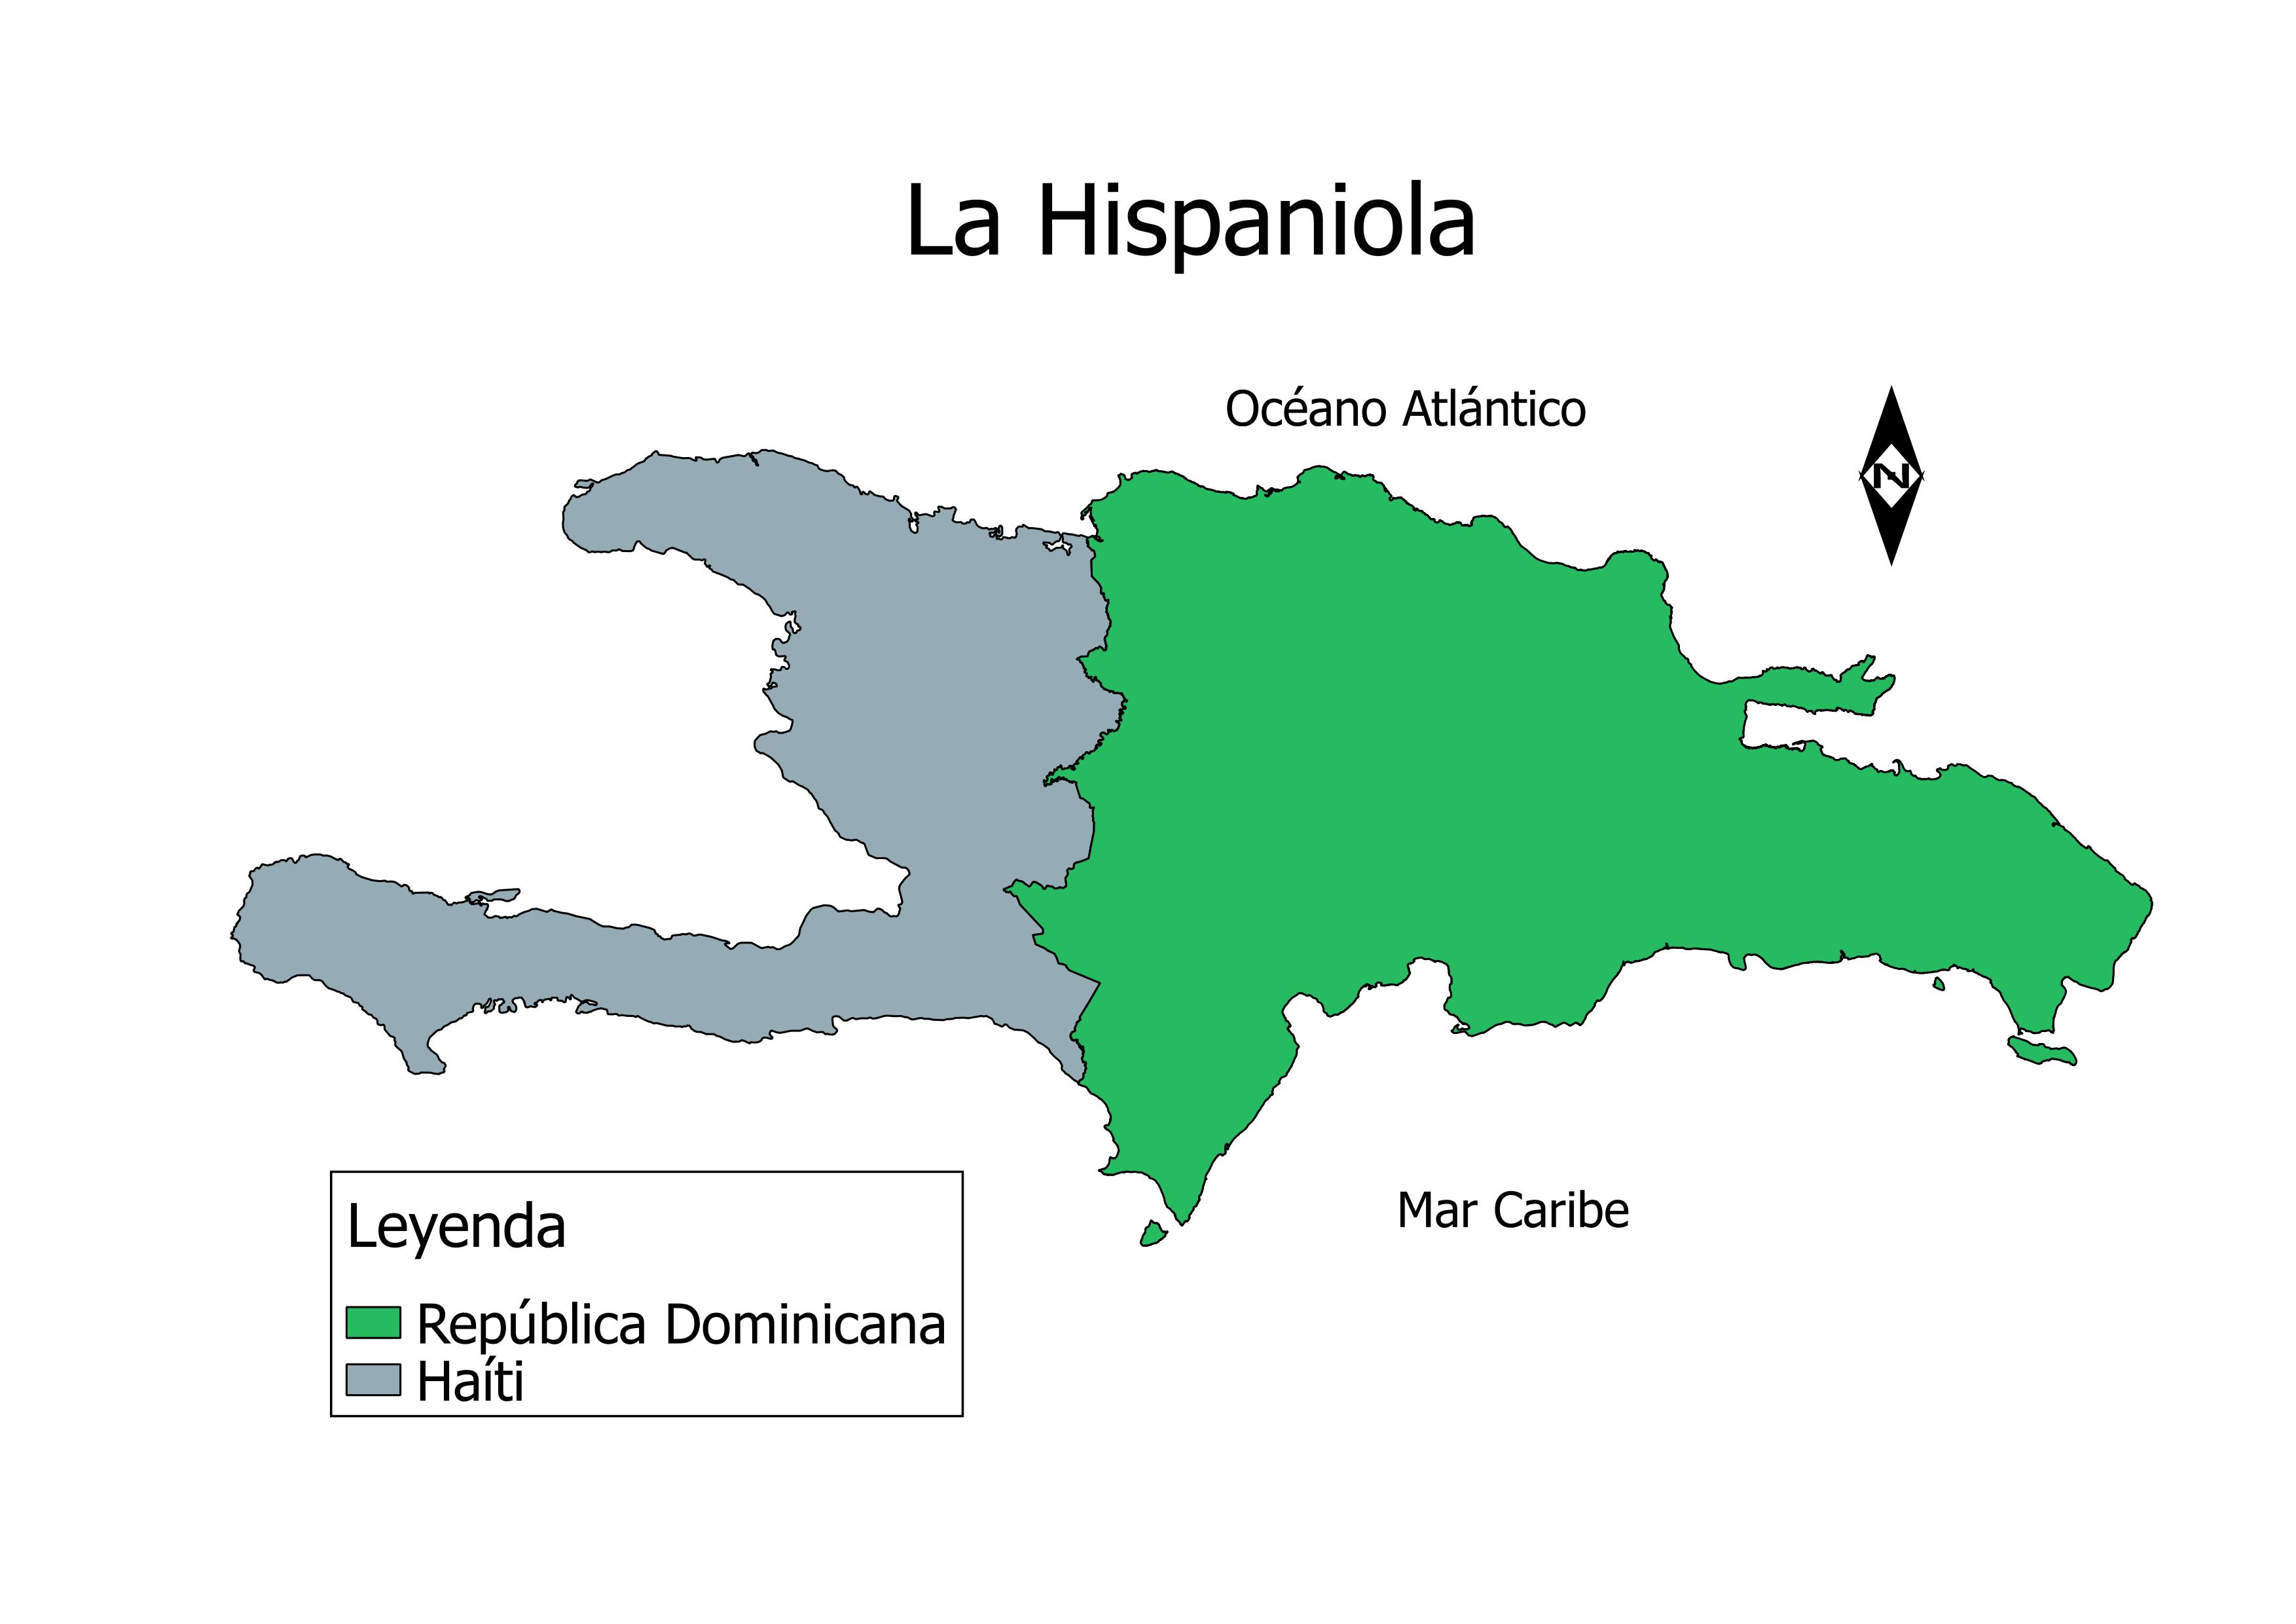
\includegraphics{La Hispan.jpeg}
\caption{La isla de la Hipaniola}
\end{figure}

Las hormigas pertenecen a una sola familia que es la Formicidae, dentro
de la superfamilia Vespoidea (RES (1993)). Forman parte de un grupo de
himenópteros sociales muy diversos, tanto taxonómica como funcionalmente
(Fernández (2001)). Las hormigas, dentro del grupo de los insectos, se
considera como uno de los grupos más evolucionados por el nivel social y
por el grado de especialización y dependencia que estas pueden alcanzar
(REYES (n.d.)).

Las hormigas representan una de las familias dominantes en cualquier
ecosistema (REYES (n.d.)). En la isla La Hispaniola se conocen 43
géneros y 147 especies y subespecies de hormigas (\emph{Ants of
hispaniola}, n.d.). No se tiene una publicación que identifique las
especies de hormigas que se encuentran dentro del campus de la UASD, ni
cómo estas se encuentran distribuidas.

Lo que se busca lograr con este informe es establecer patrones en la
distribución de las hormigas en el campus de la UASD, específicamente
para suelo y dosel. Cuando se habla de suelo en este informe hace
referencia al suelo desnudo o cubierto de grama, que no presenta
construcciones de ningún tipo, y que se encuentra bajo cielo despejado.
Mientras que cuando se habla de dosel hace referencia a suelos desnudos,
cubiertos de gramas, hojarascas o rocas, pero que estan bajo
arboles.Para analizar la similitud existente entre las parcelas se
utilizara un dendrograma, que es una representación gráfica o diagrama
de datos en forma de árbol, que se van dividiendo en subcategorías.

\section{Metodología}\label{metodologuxeda}

El campus de la UASD fue dividido en cuadriculas de 50m x 50m, formando
189 parcelas. A estas parcelas les fue asignado un tipo de suelo,
dependiendo de cual fuera el más abarcador en el área, estas
asignaciones podían ser: edificación erguida, construido, suelo y dosel
(figure 4). De estas parcelas se seleccionaron, siguiendo un muestreo
estratificado-aleatorio, 11 de suelo y 10 de dosel. Para realizar el
muestreo se tomaron 6 de las 11 de suelo y 5 de las 10 de dosel (figure
5), para un total de 11 parcelas muestreadas.

\begin{figure}
\centering
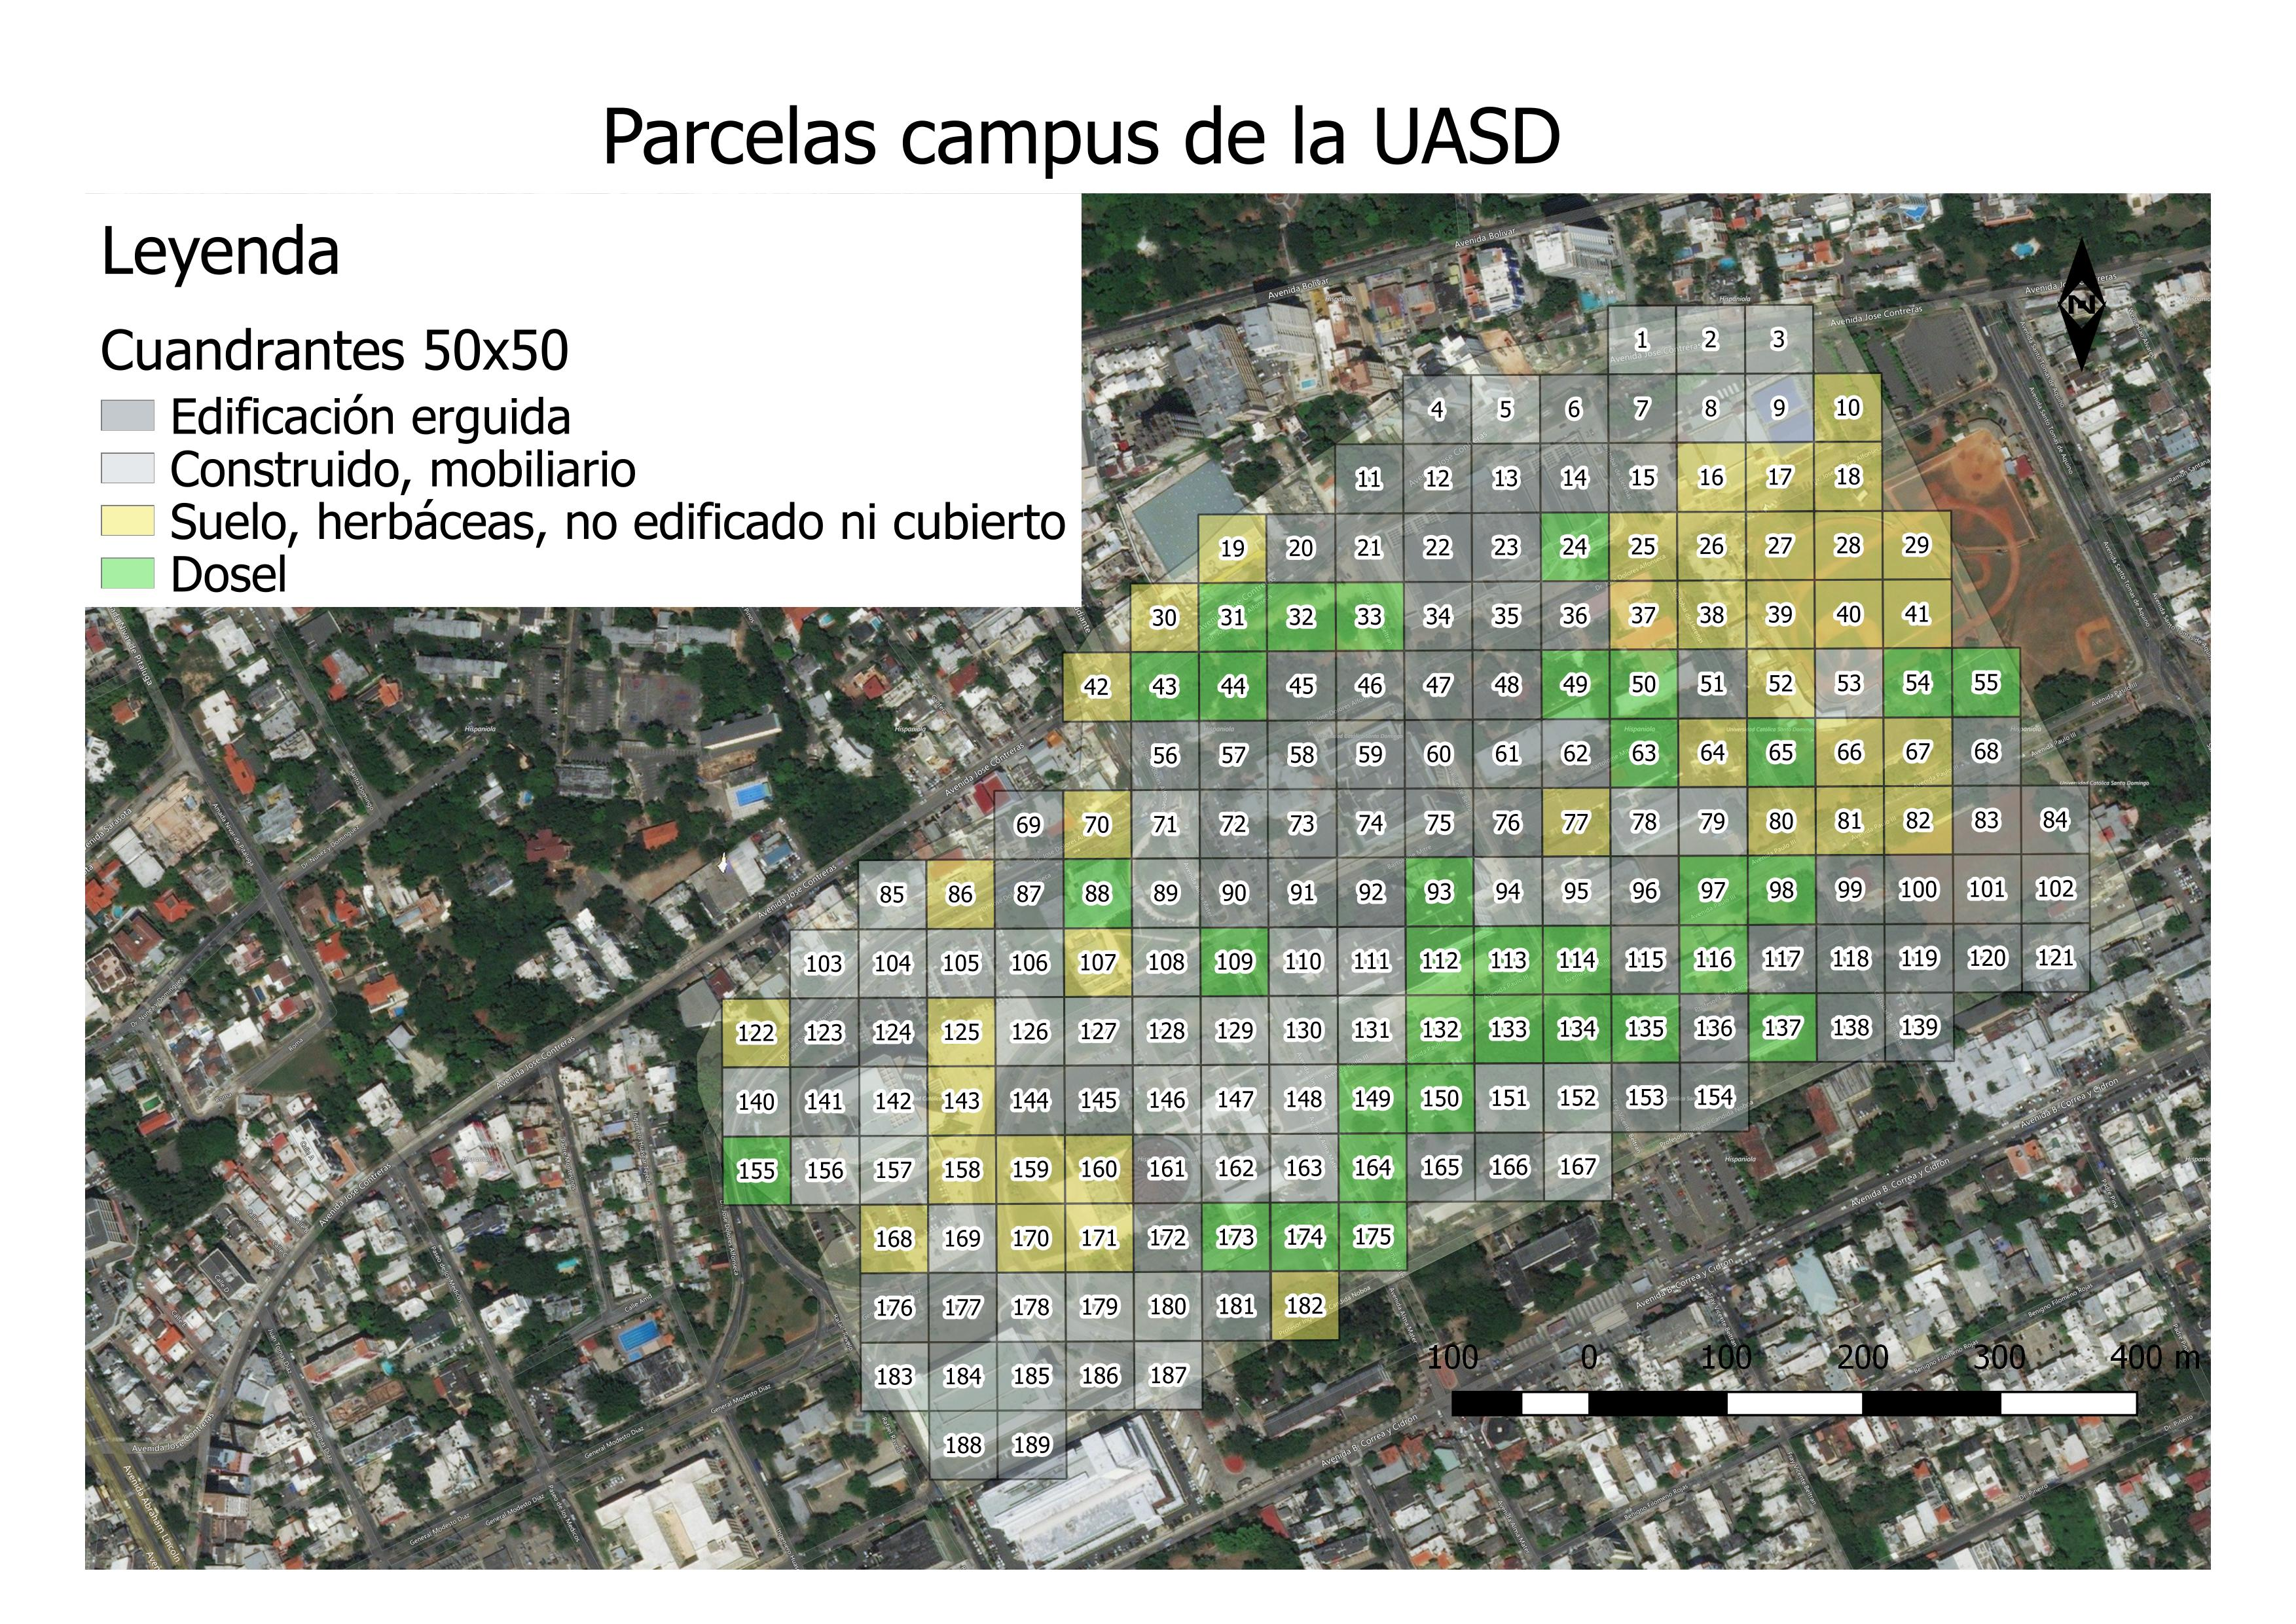
\includegraphics{parc uasd.jpeg}
\caption{}
\end{figure}

\begin{figure}
\centering
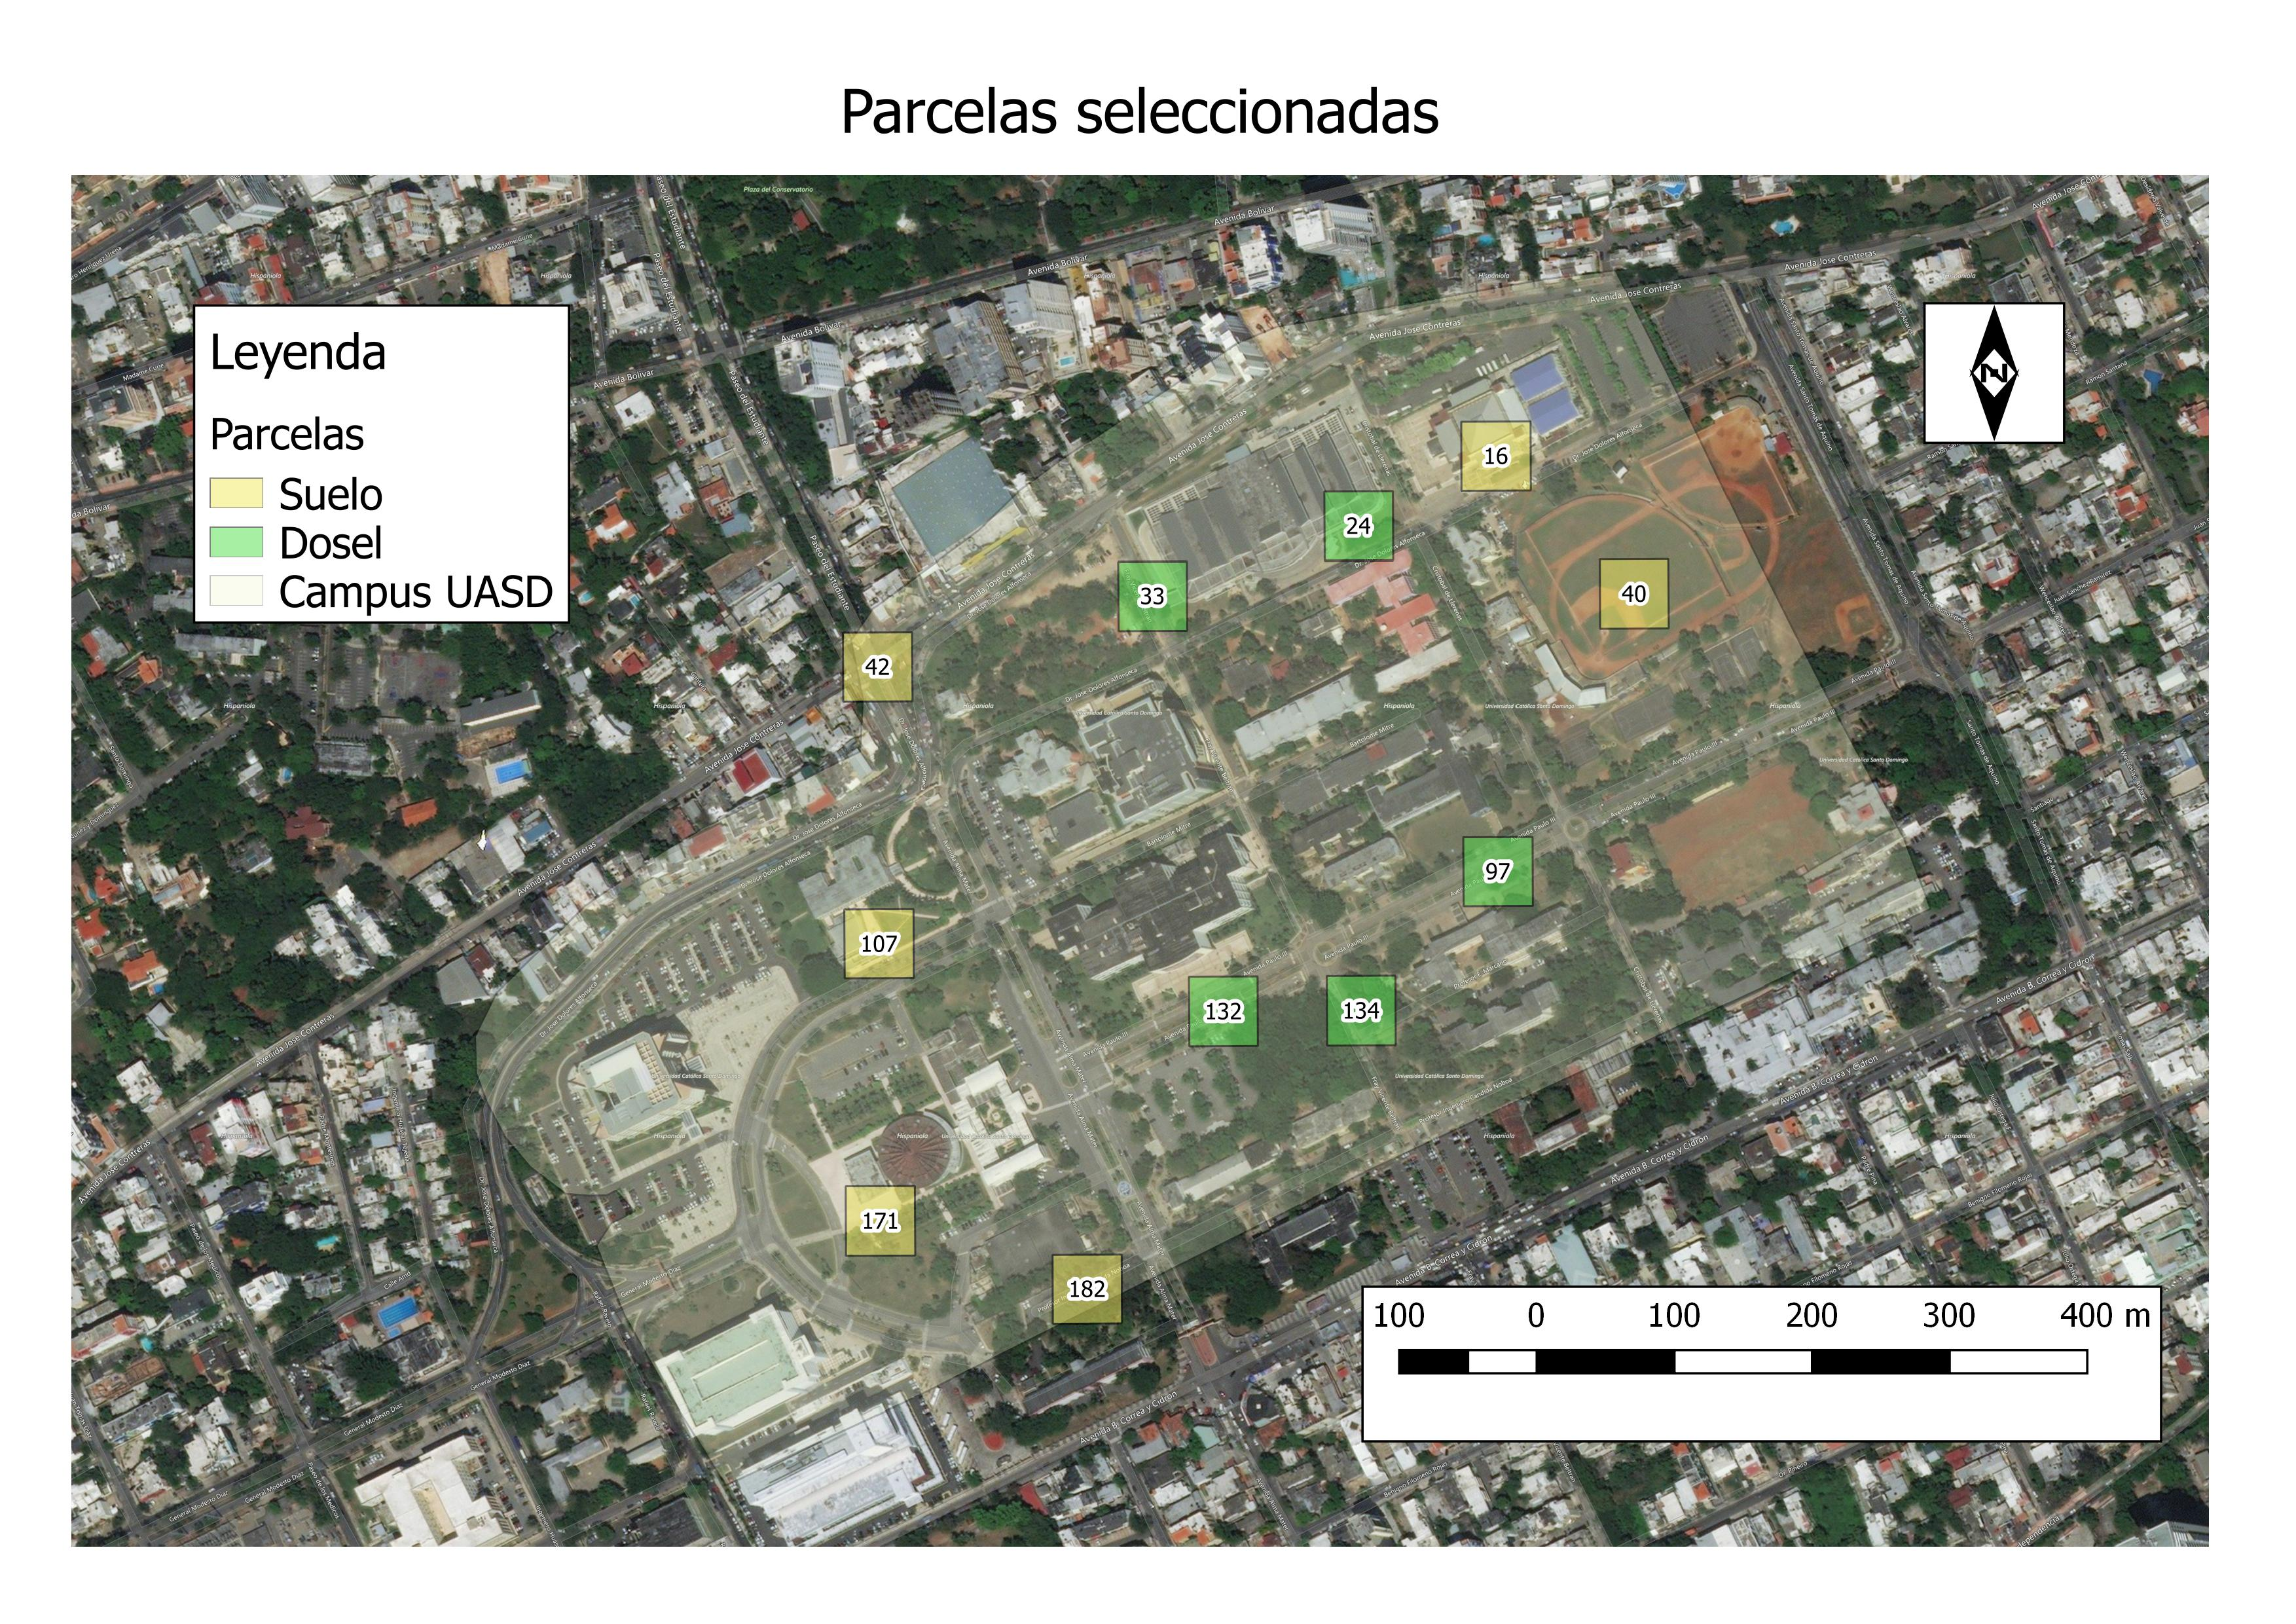
\includegraphics{parc sel.jpeg}
\caption{}
\end{figure}

Para iniciar la colecta de hormigas era necesario una lista de
materiales, entre ellos:

-ODk Collect: es una aplicación para Android que reemplaza los
formularios en papel. Se utilizó para recolectar los datos de comunidad
y ambientales de las parcelas. El formulario llenado fue el de nombre
`Hormigas UASD HABITAT'.

-Frascos para conservar las hormigas.

-Alcohol etílico al 70\%.

-Pincel para la recolección de hormigas.

-Cinta adhesiva blanca para poner los nombres en las muestras y
transparente para cubrirlos.

-Chinógrafo para escribir los códigos.

-En algunos casos, en los cuales era necesario, se utilizó la luz del
celular.

Una vez se tenían las parcelas identificadas y todos los materiales
necesarios se inició con la recolecta de hormigas. Se hacía una
cuadricula de 4x4 separa a unos 2 metros cada punto, en los cuales se
ponían los cebos (16 cebos por cada parcela); en este caso los cebos de
todas las parcelas fueron iguales, atún en aceite vegetal. Se dejaban
unos 30 minutos para que las hormigas llegaran, mientras tanto se
llenaba el formulario de ODK Collect.

Una vez pasados los 30 minutos se iniciaba a recolectar las hormigas,
para lo cual se tomaban del cebo con el pincel y se llevaban a los
frascos llenos de alcohol etílico. Este frasco era identificado con un
código único, el cual también era el código registrado en el ODk
Collect. Todos los individuos encontrado en la misma parcela se
depositaban en un mismo frasco.

Luego de recoger las 11 muestras se identificaron utilizando una lupa
electrónica y un formulario de identificación que se encuentra en
(\emph{Ants of hispaniola}, n.d.).

\section{Resultados}\label{resultados}

\subsection{Carga de funciones y
paquetes}\label{carga-de-funciones-y-paquetes}

\begin{Shaded}
\begin{Highlighting}[]
\KeywordTok{library}\NormalTok{(tidyverse)}
\KeywordTok{library}\NormalTok{(knitr)}
\KeywordTok{library}\NormalTok{(sf)}
\KeywordTok{library}\NormalTok{(vegan)}
\KeywordTok{library}\NormalTok{(ade4)}
\KeywordTok{library}\NormalTok{(FactoMineR)}
\KeywordTok{library}\NormalTok{(readr)}
\KeywordTok{source}\NormalTok{(}\StringTok{'src/funciones_analisis.R'}\NormalTok{)}
\end{Highlighting}
\end{Shaded}

\subsection{Hormigas encontradas en el campus de la
UASD.}\label{hormigas-encontradas-en-el-campus-de-la-uasd.}

\begin{longtable}[]{@{}lc@{}}
\toprule
Subfamilia & Género\tabularnewline
\midrule
\endhead
Myrmicinae & Cardiocondyla sp\tabularnewline
& Monomorium sp\tabularnewline
& Pheidole sp\tabularnewline
& Solenopsis s\tabularnewline
& Tetramorium sp\tabularnewline
& Wasmannia sp\tabularnewline
Formicinae & Brachymyrmex sp,\tabularnewline
& Paratrechina sp\tabularnewline
Dolichoderinae & Dorymyrmex sp\tabularnewline
Pseudomyrmecinae & Pseudomyrmex sp\tabularnewline
\bottomrule
\end{longtable}

-Género en suelo = 7

-Género en dosel = 10

\subsection{Tablas y gráficos}\label{tablas-y-gruxe1ficos}

\begin{Shaded}
\begin{Highlighting}[]
\NormalTok{todos_los_habitat <-}\StringTok{ }\KeywordTok{read.csv}\NormalTok{(}\StringTok{'export/tabla_todos_los_habitat.csv'}\NormalTok{)}
\NormalTok{todos_los_nidos <-}\StringTok{ }\KeywordTok{read.csv}\NormalTok{(}\StringTok{'export/tabla_todos_los_nidos.csv'}\NormalTok{)}
\NormalTok{mcpooledhabitat <-}\StringTok{ }\KeywordTok{read.csv}\NormalTok{(}\StringTok{'export/mc_pooled_habitat.csv'}\NormalTok{, }\DataTypeTok{row.names =} \DecValTok{1}\NormalTok{)}
\NormalTok{mcpoolednidos <-}\StringTok{ }\KeywordTok{read.csv}\NormalTok{(}\StringTok{'export/mc_pooled_nidos.csv'}\NormalTok{, }\DataTypeTok{row.names =} \DecValTok{1}\NormalTok{)}
\NormalTok{nomlat <-}\StringTok{ }\KeywordTok{read_csv}\NormalTok{(}\StringTok{'equivalencia_etiqueta_nombre_latino.csv'}\NormalTok{)}
\end{Highlighting}
\end{Shaded}

\begin{Shaded}
\begin{Highlighting}[]
\NormalTok{mcemdilone <-}\StringTok{ }\KeywordTok{matriz_comunidad_hab}\NormalTok{(}\StringTok{'emdilone'}\NormalTok{)}
\NormalTok{maemdilone <-}\StringTok{ }\KeywordTok{matriz_ambiental_hab}\NormalTok{(}\StringTok{'emdilone'}\NormalTok{)}
\NormalTok{maemdilone <-}\StringTok{ }\NormalTok{maemdilone[}\KeywordTok{match}\NormalTok{(}\KeywordTok{rownames}\NormalTok{(mcemdilone), }\KeywordTok{rownames}\NormalTok{(maemdilone)),]}
\end{Highlighting}
\end{Shaded}

\subsection{Análisis exploratorios
básicos:}\label{anuxe1lisis-exploratorios-buxe1sicos}

Matriz de Comunidad

\begin{Shaded}
\begin{Highlighting}[]
\NormalTok{mcemdilone }\OperatorTok\StringTok{ }\NormalTok{kable}
\end{Highlighting}
\end{Shaded}

\begin{longtable}[]{@{}lrrrrrrrrrr@{}}
\toprule
& Brachymyrmex & Cardiocondyla & Dorymyrmex & Monomorium & Paratrechina
& Pheidole & Pseudomyrmex & Solenopsis & Tetramorium &
Wasmannia\tabularnewline
\midrule
\endhead
p107 & 0 & 1 & 1 & 0 & 0 & 1 & 0 & 1 & 0 & 0\tabularnewline
p132 & 0 & 0 & 1 & 0 & 0 & 1 & 1 & 1 & 1 & 0\tabularnewline
p134 & 1 & 1 & 0 & 0 & 0 & 1 & 0 & 1 & 0 & 0\tabularnewline
p16 & 1 & 0 & 1 & 0 & 0 & 0 & 0 & 0 & 0 & 0\tabularnewline
p171 & 1 & 0 & 1 & 0 & 0 & 0 & 0 & 1 & 0 & 0\tabularnewline
p182 & 0 & 0 & 1 & 1 & 0 & 1 & 0 & 0 & 0 & 0\tabularnewline
p24 & 1 & 1 & 1 & 0 & 1 & 1 & 0 & 0 & 1 & 0\tabularnewline
p33 & 1 & 1 & 1 & 0 & 0 & 1 & 0 & 1 & 0 & 1\tabularnewline
p40 & 0 & 0 & 0 & 0 & 0 & 0 & 0 & 1 & 0 & 0\tabularnewline
p42 & 1 & 0 & 1 & 0 & 1 & 0 & 0 & 1 & 0 & 0\tabularnewline
p97 & 1 & 0 & 0 & 1 & 0 & 1 & 0 & 0 & 0 & 0\tabularnewline
\bottomrule
\end{longtable}

Matriz ambiental

\begin{Shaded}
\begin{Highlighting}[]
\NormalTok{maemdilone }\OperatorTok\StringTok{ }\NormalTok{kable}
\end{Highlighting}
\end{Shaded}

\begin{longtable}[]{@{}lllllllllllllllllr@{}}
\toprule
& horainicio & horafinal & distanciaabasura & distanciaagua &
distanciavias & actividadpersonas & actividadcebo1 & actividadcebo2 &
actividadcebo3 & actividadcebo4 & fechacolecta & plantas & cebosbajo &
cebossobre & cebosotrosele & tipo & riqueza\tabularnewline
\midrule
\endhead
p107 & 4.14 pm & 5.29 pm & 10omas & no hay a la vista & 1a5 & 0 & 6a9 &
1a5 & 0 & 1a5 & 2019-10-13T00:00:00Z & Mango & despejado & hierba &
hojarasca & suelo, herbáceas, no edificado ni cubierto &
4\tabularnewline
p132 & 3.35 pm & 4.56 pm & 1a5 & no hay a la vista & 1a5 & 0 & 10omas &
10omas & 10omas & 10omas & 2019-10-26T00:00:00Z & Nin & dosel &
suelo\_tierra & hojarasca,basura\_restos\_comida,ramas\_troncos & dosel
& 5\tabularnewline
p134 & 11.24 am & 12.51 pm & 10omas & no hay a la vista & 1a5 & 0 &
10omas & 10omas & 10omas & 10omas & 2019-10-24T00:00:00Z & Palma & dosel
& hierba,suelo\_tierra & hojarasca & dosel & 4\tabularnewline
p16 & 10.28 am & 11.38 am & 10omas & no\_aplica & 1a5 & 1a5 & 1a5 &
10omas & 0 & 1a5 & 2019-10-12T00:00:00Z & Mango, coco & despejado &
hierba & no\_aplica & suelo, herbáceas, no edificado ni cubierto &
2\tabularnewline
p171 & 2.03 pm & 3.04 pm & 1a5 & no hay a la vista & 1a5 & 0 & 10omas &
10omas & 10omas & 10omas & 2019-10-14T00:00:00Z & Framboyan, pino, palma
& despejado & hierba & hojarasca & suelo, herbáceas, no edificado ni
cubierto & 3\tabularnewline
p182 & 4.47 pm & 6.15 pm & 10omas & no hay a la vista & 1a5 & 0 & 10omas
& 6a9 & 10omas & 10omas & 2019-09-27T00:00:00Z & NULL & despejado &
hierba & hojarasca,basura\_restos\_comida & suelo, herbáceas, no
edificado ni cubierto & 3\tabularnewline
p24 & 3.03 pm & 5.57 pm & 1a5 & no hay a la vista & 1a5 & 0 & 10omas &
10omas & 10omas & 10omas & 2019-10-13T00:00:00Z & Almendra & dosel &
no\_aplica & hojarasca,rocas & dosel & 6\tabularnewline
p33 & 11.43 am & 12.51 pm & 10omas & no hay a la vista & 1a5 & 0 &
10omas & 10omas & 10omas & 10omas & 2019-10-25T00:00:00Z & NULL & dosel
& suelo\_tierra,hierba & hojarasca,ramas\_troncos & dosel &
6\tabularnewline
p40 & 12.06 pm & 12.57 pm & 6a9 & no hay a la vista & 1a5 & 0 & 0 & 0 &
10omas & 0 & 2019-10-12T00:00:00Z & NULL & despejado & hierba &
basura\_restos\_comida & suelo, herbáceas, no edificado ni cubierto &
1\tabularnewline
p42 & 10.14 am & 11.32 am & 10omas & no hay a la vista & 6a9 & 0 &
10omas & 10omas & 10omas & 10omas & 2019-10-25T00:00:00Z & NULL &
despejado & hierba,suelo\_tierra &
hojarasca,ramas\_troncos,rocas,basura\_restos\_comida & suelo,
herbáceas, no edificado ni cubierto & 4\tabularnewline
p97 & 3.40 pm & 4.51 pm & 1a5 & no hay a la vista & 1a5 & no\_aplica &
10omas & 10omas & 6a9 & 10omas & 2019-10-14T00:00:00Z & Pino, framboyan
& dosel & hierba & hojarasca & dosel & 3\tabularnewline
\bottomrule
\end{longtable}

Número de géneros por parcela

\begin{Shaded}
\begin{Highlighting}[]
\NormalTok{mcemdilone }\OperatorTok\StringTok{ }\NormalTok{specnumber }\OperatorTok\StringTok{ }\NormalTok{sort }\OperatorTok\StringTok{ }\NormalTok{kable}
\end{Highlighting}
\end{Shaded}

\begin{longtable}[]{@{}lr@{}}
\toprule
& x\tabularnewline
\midrule
\endhead
p40 & 1\tabularnewline
p16 & 2\tabularnewline
p171 & 3\tabularnewline
p182 & 3\tabularnewline
p97 & 3\tabularnewline
p107 & 4\tabularnewline
p134 & 4\tabularnewline
p42 & 4\tabularnewline
p132 & 5\tabularnewline
p24 & 6\tabularnewline
p33 & 6\tabularnewline
\bottomrule
\end{longtable}

Número de parcelas según conteo de género

\begin{Shaded}
\begin{Highlighting}[]
\NormalTok{mcemdilone }\OperatorTok\StringTok{ }\NormalTok{rowSums }\OperatorTok\StringTok{ }\NormalTok{table }\OperatorTok\StringTok{ }\NormalTok{kable}
\end{Highlighting}
\end{Shaded}

\begin{longtable}[]{@{}lr@{}}
\toprule
. & Freq\tabularnewline
\midrule
\endhead
1 & 1\tabularnewline
2 & 1\tabularnewline
3 & 3\tabularnewline
4 & 3\tabularnewline
5 & 1\tabularnewline
6 & 2\tabularnewline
\bottomrule
\end{longtable}

Número de parcelas en las que aparece cada género

\begin{Shaded}
\begin{Highlighting}[]
\NormalTok{mcemdilone }\OperatorTok\StringTok{ }\NormalTok{colSums }\OperatorTok\StringTok{ }\NormalTok{sort }\OperatorTok\StringTok{ }\NormalTok{kable}
\end{Highlighting}
\end{Shaded}

\begin{longtable}[]{@{}lr@{}}
\toprule
& x\tabularnewline
\midrule
\endhead
Pseudomyrmex & 1\tabularnewline
Wasmannia & 1\tabularnewline
Monomorium & 2\tabularnewline
Paratrechina & 2\tabularnewline
Tetramorium & 2\tabularnewline
Cardiocondyla & 4\tabularnewline
Brachymyrmex & 7\tabularnewline
Pheidole & 7\tabularnewline
Solenopsis & 7\tabularnewline
Dorymyrmex & 8\tabularnewline
\bottomrule
\end{longtable}

Número de parcelas en las que aparece cada genero, por tipo de parcela

\begin{longtable}[]{@{}lcc@{}}
\toprule
Especie & Suelo & Dosel\tabularnewline
\midrule
\endhead
Brachymyrmex sp & 3 & 4\tabularnewline
Cardiocondyla sp & 1 & 3\tabularnewline
Dorymyrmex sp & 5 & 3\tabularnewline
Monomorium sp & 1 & 1\tabularnewline
Paratrechina sp & 1 & 1\tabularnewline
Pheidole sp & 2 & 5\tabularnewline
Pseudomyrmex sp & 0 & 1\tabularnewline
Solenopsis sp & 4 & 3\tabularnewline
Tetramorium sp & 0 & 2\tabularnewline
Wasmannia sp & 0 & 1\tabularnewline
\bottomrule
\end{longtable}

\subsection{Curva de acumulación de
especies:}\label{curva-de-acumulaciuxf3n-de-especies}

\begin{Shaded}
\begin{Highlighting}[]
\NormalTok{mcemdilone_sac <-}\StringTok{ }\KeywordTok{specaccum}\NormalTok{(mcemdilone)}
\KeywordTok{plot}\NormalTok{(mcemdilone_sac, }\DataTypeTok{ci.type=}\StringTok{"polygon"}\NormalTok{, }\DataTypeTok{ci.col=}\StringTok{"yellow"}\NormalTok{)  }
\end{Highlighting}
\end{Shaded}

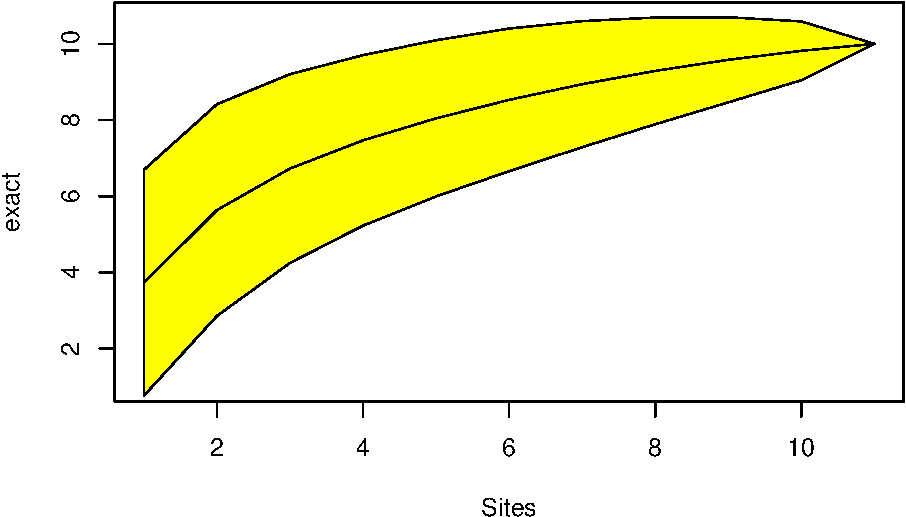
\includegraphics{manuscrito_files/figure-latex/curva_acumulacion_emdilone-1.pdf}

\subsection{Ordenación: dendrograma y
PCoA}\label{ordenaciuxf3n-dendrograma-y-pcoa}

Generar matrices de comunidad y ambiental para ordenación:

\begin{Shaded}
\begin{Highlighting}[]
\NormalTok{mcem_ord <-}\StringTok{ }\KeywordTok{mc_para_ord}\NormalTok{(}\DataTypeTok{filtusuario =} \StringTok{'emdilone'}\NormalTok{)}
\NormalTok{mcem_ord }\OperatorTok\StringTok{ }\NormalTok{kable}
\end{Highlighting}
\end{Shaded}

\begin{longtable}[]{@{}lrrrrrrrrrr@{}}
\toprule
& Brachymyrmex & Cardiocondyla & Dorymyrmex & Monomorium & Paratrechina
& Pheidole & Pseudomyrmex & Solenopsis & Tetramorium &
Wasmannia\tabularnewline
\midrule
\endhead
p107 & 0.0000000 & 0.5000000 & 0.5000000 & 0.0000000 & 0.0000000 &
0.5000000 & 0.0000000 & 0.5000000 & 0.0000000 & 0.0000000\tabularnewline
p132 & 0.0000000 & 0.0000000 & 0.4472136 & 0.0000000 & 0.0000000 &
0.4472136 & 0.4472136 & 0.4472136 & 0.4472136 & 0.0000000\tabularnewline
p134 & 0.5000000 & 0.5000000 & 0.0000000 & 0.0000000 & 0.0000000 &
0.5000000 & 0.0000000 & 0.5000000 & 0.0000000 & 0.0000000\tabularnewline
p16 & 0.7071068 & 0.0000000 & 0.7071068 & 0.0000000 & 0.0000000 &
0.0000000 & 0.0000000 & 0.0000000 & 0.0000000 & 0.0000000\tabularnewline
p171 & 0.5773503 & 0.0000000 & 0.5773503 & 0.0000000 & 0.0000000 &
0.0000000 & 0.0000000 & 0.5773503 & 0.0000000 & 0.0000000\tabularnewline
p182 & 0.0000000 & 0.0000000 & 0.5773503 & 0.5773503 & 0.0000000 &
0.5773503 & 0.0000000 & 0.0000000 & 0.0000000 & 0.0000000\tabularnewline
p24 & 0.4082483 & 0.4082483 & 0.4082483 & 0.0000000 & 0.4082483 &
0.4082483 & 0.0000000 & 0.0000000 & 0.4082483 & 0.0000000\tabularnewline
p33 & 0.4082483 & 0.4082483 & 0.4082483 & 0.0000000 & 0.0000000 &
0.4082483 & 0.0000000 & 0.4082483 & 0.0000000 & 0.4082483\tabularnewline
p40 & 0.0000000 & 0.0000000 & 0.0000000 & 0.0000000 & 0.0000000 &
0.0000000 & 0.0000000 & 1.0000000 & 0.0000000 & 0.0000000\tabularnewline
p42 & 0.5000000 & 0.0000000 & 0.5000000 & 0.0000000 & 0.5000000 &
0.0000000 & 0.0000000 & 0.5000000 & 0.0000000 & 0.0000000\tabularnewline
p97 & 0.5773503 & 0.0000000 & 0.0000000 & 0.5773503 & 0.0000000 &
0.5773503 & 0.0000000 & 0.0000000 & 0.0000000 & 0.0000000\tabularnewline
\bottomrule
\end{longtable}

\begin{Shaded}
\begin{Highlighting}[]
\NormalTok{maem_ord <-}\StringTok{ }\KeywordTok{ma_para_ord}\NormalTok{(}\DataTypeTok{filtusuario =} \StringTok{'emdilone'}\NormalTok{, }\DataTypeTok{mc =}\NormalTok{ mcem_ord)}
\NormalTok{maem_ord }\OperatorTok\StringTok{ }\NormalTok{kable}
\end{Highlighting}
\end{Shaded}

\begin{longtable}[]{@{}lrllllllllllll@{}}
\toprule
& riqueza & tipo & distanciaabasura & distanciaagua & distanciavias &
actividadpersonas & actividadcebo1 & actividadcebo2 & actividadcebo3 &
actividadcebo4 & cebosbajo & cebossobre & cebosotrosele\tabularnewline
\midrule
\endhead
p107 & 4 & suelo, herbáceas, no edificado ni cubierto & 10omas & no hay
a la vista & 1a5 & 0 & 6a9 & 1a5 & 0 & 1a5 & despejado & hierba &
hojarasca\tabularnewline
p132 & 5 & dosel & 1a5 & no hay a la vista & 1a5 & 0 & 10omas & 10omas &
10omas & 10omas & dosel & suelo\_tierra &
hojarasca,basura\_restos\_comida,ramas\_troncos\tabularnewline
p134 & 4 & dosel & 10omas & no hay a la vista & 1a5 & 0 & 10omas &
10omas & 10omas & 10omas & dosel & hierba,suelo\_tierra &
hojarasca\tabularnewline
p16 & 2 & suelo, herbáceas, no edificado ni cubierto & 10omas &
no\_aplica & 1a5 & 1a5 & 1a5 & 10omas & 0 & 1a5 & despejado & hierba &
no\_aplica\tabularnewline
p171 & 3 & suelo, herbáceas, no edificado ni cubierto & 1a5 & no hay a
la vista & 1a5 & 0 & 10omas & 10omas & 10omas & 10omas & despejado &
hierba & hojarasca\tabularnewline
p182 & 3 & suelo, herbáceas, no edificado ni cubierto & 10omas & no hay
a la vista & 1a5 & 0 & 10omas & 6a9 & 10omas & 10omas & despejado &
hierba & hojarasca,basura\_restos\_comida\tabularnewline
p24 & 6 & dosel & 1a5 & no hay a la vista & 1a5 & 0 & 10omas & 10omas &
10omas & 10omas & dosel & no\_aplica & hojarasca,rocas\tabularnewline
p33 & 6 & dosel & 10omas & no hay a la vista & 1a5 & 0 & 10omas & 10omas
& 10omas & 10omas & dosel & suelo\_tierra,hierba &
hojarasca,ramas\_troncos\tabularnewline
p40 & 1 & suelo, herbáceas, no edificado ni cubierto & 6a9 & no hay a la
vista & 1a5 & 0 & 0 & 0 & 10omas & 0 & despejado & hierba &
basura\_restos\_comida\tabularnewline
p42 & 4 & suelo, herbáceas, no edificado ni cubierto & 10omas & no hay a
la vista & 6a9 & 0 & 10omas & 10omas & 10omas & 10omas & despejado &
hierba,suelo\_tierra &
hojarasca,ramas\_troncos,rocas,basura\_restos\_comida\tabularnewline
p97 & 3 & dosel & 1a5 & no hay a la vista & 1a5 & no\_aplica & 10omas &
10omas & 6a9 & 10omas & dosel & hierba & hojarasca\tabularnewline
\bottomrule
\end{longtable}

\subsubsection{Dendrograma}\label{dendrograma}

\begin{Shaded}
\begin{Highlighting}[]
\KeywordTok{dendro}\NormalTok{(}\DataTypeTok{mc =}\NormalTok{ mcem_ord, }\DataTypeTok{k =} \DecValTok{4}\NormalTok{)}
\end{Highlighting}
\end{Shaded}

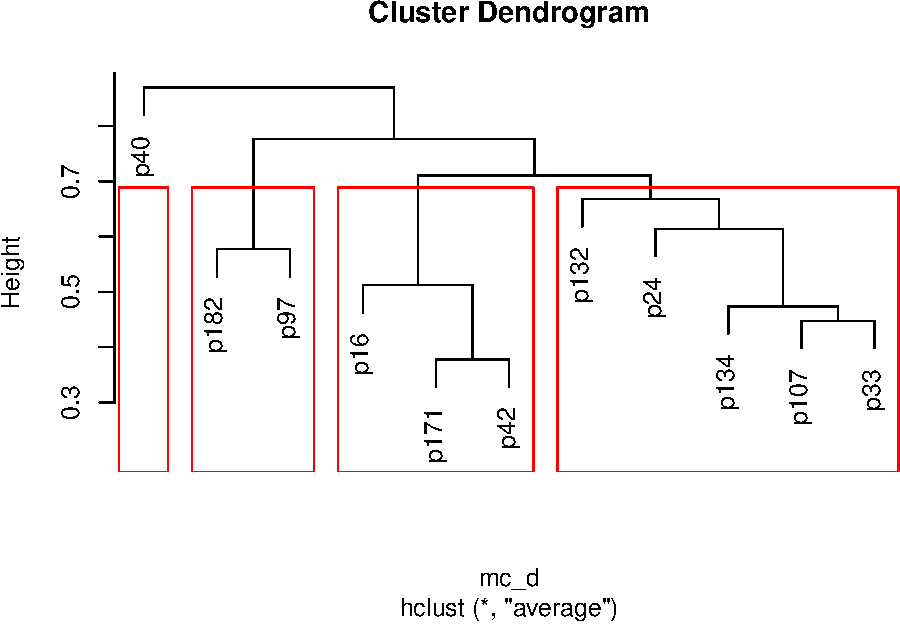
\includegraphics{manuscrito_files/figure-latex/dendro_emdilone-1.pdf}

*Grupo 1

\begin{Shaded}
\begin{Highlighting}[]
\NormalTok{mcemdilone[}\KeywordTok{c}\NormalTok{(}\StringTok{'p40'}\NormalTok{),] }\OperatorTok\StringTok{ }\NormalTok{kable}
\end{Highlighting}
\end{Shaded}

\begin{longtable}[]{@{}lrrrrrrrrrr@{}}
\toprule
& Brachymyrmex & Cardiocondyla & Dorymyrmex & Monomorium & Paratrechina
& Pheidole & Pseudomyrmex & Solenopsis & Tetramorium &
Wasmannia\tabularnewline
\midrule
\endhead
p40 & 0 & 0 & 0 & 0 & 0 & 0 & 0 & 1 & 0 & 0\tabularnewline
\bottomrule
\end{longtable}

La parcela 40 se encontró un solo género, Solenopsis.

*Grupo 2

\begin{Shaded}
\begin{Highlighting}[]
\NormalTok{mcemdilone[}\KeywordTok{c}\NormalTok{(}\StringTok{'p182'}\NormalTok{, }\StringTok{'p97'}\NormalTok{),] }\OperatorTok\StringTok{ }\NormalTok{kable}
\end{Highlighting}
\end{Shaded}

\begin{longtable}[]{@{}lrrrrrrrrrr@{}}
\toprule
& Brachymyrmex & Cardiocondyla & Dorymyrmex & Monomorium & Paratrechina
& Pheidole & Pseudomyrmex & Solenopsis & Tetramorium &
Wasmannia\tabularnewline
\midrule
\endhead
p182 & 0 & 0 & 1 & 1 & 0 & 1 & 0 & 0 & 0 & 0\tabularnewline
p97 & 1 & 0 & 0 & 1 & 0 & 1 & 0 & 0 & 0 & 0\tabularnewline
\bottomrule
\end{longtable}

En las parcelas 182 y 97 se encontraron 3 géneros, de los cuales tienen
2 en común, Monomorium y Pheidole.

*Grupo 3

\begin{Shaded}
\begin{Highlighting}[]
\NormalTok{mcemdilone[}\KeywordTok{c}\NormalTok{(}\StringTok{'p16'}\NormalTok{, }\StringTok{'p171'}\NormalTok{, }\StringTok{'p42'}\NormalTok{),] }\OperatorTok\StringTok{ }\NormalTok{kable}
\end{Highlighting}
\end{Shaded}

\begin{longtable}[]{@{}lrrrrrrrrrr@{}}
\toprule
& Brachymyrmex & Cardiocondyla & Dorymyrmex & Monomorium & Paratrechina
& Pheidole & Pseudomyrmex & Solenopsis & Tetramorium &
Wasmannia\tabularnewline
\midrule
\endhead
p16 & 1 & 0 & 1 & 0 & 0 & 0 & 0 & 0 & 0 & 0\tabularnewline
p171 & 1 & 0 & 1 & 0 & 0 & 0 & 0 & 1 & 0 & 0\tabularnewline
p42 & 1 & 0 & 1 & 0 & 1 & 0 & 0 & 1 & 0 & 0\tabularnewline
\bottomrule
\end{longtable}

En las parcelas 16, 171 y 42 están presente Brachymyrmex y Dorymyrmex.

*Grupo 4

\begin{Shaded}
\begin{Highlighting}[]
\NormalTok{mcemdilone[}\KeywordTok{c}\NormalTok{(}\StringTok{'p132'}\NormalTok{, }\StringTok{'p24'}\NormalTok{, }\StringTok{'p134'}\NormalTok{, }\StringTok{'p107'}\NormalTok{, }\StringTok{'p33'}\NormalTok{),] }\OperatorTok\StringTok{ }\NormalTok{kable}
\end{Highlighting}
\end{Shaded}

\begin{longtable}[]{@{}lrrrrrrrrrr@{}}
\toprule
& Brachymyrmex & Cardiocondyla & Dorymyrmex & Monomorium & Paratrechina
& Pheidole & Pseudomyrmex & Solenopsis & Tetramorium &
Wasmannia\tabularnewline
\midrule
\endhead
p132 & 0 & 0 & 1 & 0 & 0 & 1 & 1 & 1 & 1 & 0\tabularnewline
p24 & 1 & 1 & 1 & 0 & 1 & 1 & 0 & 0 & 1 & 0\tabularnewline
p134 & 1 & 1 & 0 & 0 & 0 & 1 & 0 & 1 & 0 & 0\tabularnewline
p107 & 0 & 1 & 1 & 0 & 0 & 1 & 0 & 1 & 0 & 0\tabularnewline
p33 & 1 & 1 & 1 & 0 & 0 & 1 & 0 & 1 & 0 & 1\tabularnewline
\bottomrule
\end{longtable}

En las parcelas 132, 24, 134, 107 y 33 tienen en común a Pheidole.

\subsubsection{PCoA:}\label{pcoa}

\begin{Shaded}
\begin{Highlighting}[]
\NormalTok{pcoa_em <-}\StringTok{ }\KeywordTok{pcoagg}\NormalTok{(}\DataTypeTok{mc =}\NormalTok{ mcem_ord, }\DataTypeTok{ma =}\NormalTok{ maem_ord, }\DataTypeTok{distmethod =} \StringTok{'gower'}\NormalTok{, }\DataTypeTok{textoetiq =} \DecValTok{2}\NormalTok{, }\DataTypeTok{p_max =} \FloatTok{0.2}\NormalTok{)}
\NormalTok{pcoa_em[}\StringTok{'grafico'}\NormalTok{]}
\NormalTok{## $grafico}
\end{Highlighting}
\end{Shaded}

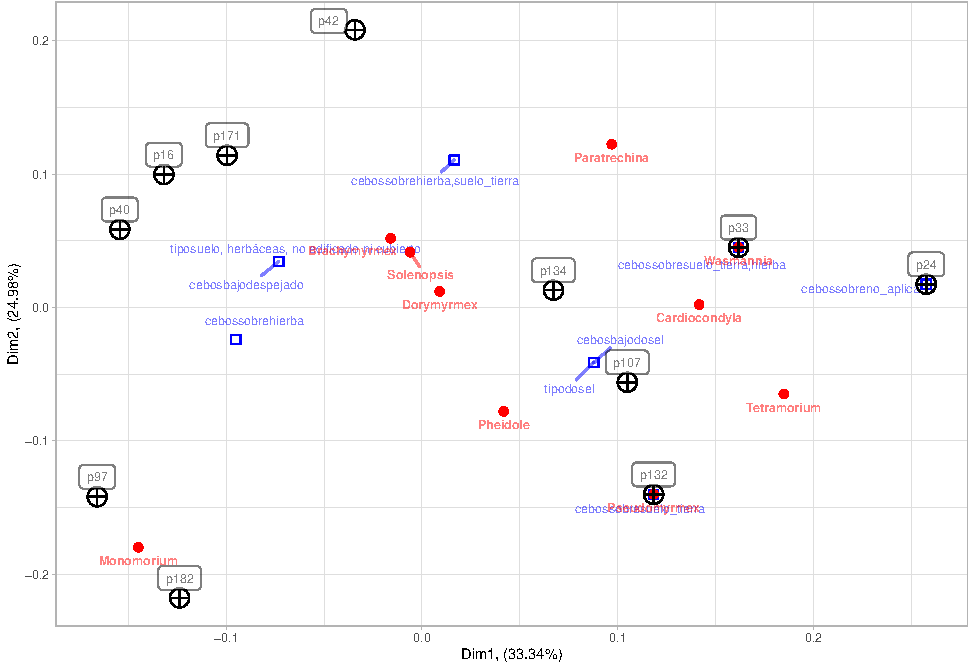
\includegraphics[width=1500px]{manuscrito_files/figure-latex/pcoa_emdilone-1}

\section{Discusión}\label{discusiuxf3n}

En las 11 parcelas muestreadas se encontraron 10 géneros de hormigas. En
suelo se encontraron 7 de los 10 y en dosel los 10 en total. La más
común fue Dorymyrmex sp, la cual se encontró en 8 de las 11 parcelas,
seguida por Solenopsis sp, Pheidole sp. y Brachymyrmex sp, las cuales
aparecen en 7 de las 11 parcelas. Las menos comunes fueron Pseudomyrmex
y Wasmania, solo se encontraron en 1 de las 11 parcelas.

Pseudomyrmex sp, Tetramorium sp y Wasmannia sp fueron encontradas solo
en parcelas de dosel. Pseudomyrmex es una hormiga arbórea, por lo cual
no es común encontrarla en cebos; lo que se estima es que, ya que, el
cebo se encontraba colocado bojo cobertura de arboles, la misma cayó
desde el arbol durante la muestra, lo que no se explica es si fue
coincidencia o si la misma se sintió atraida por el cebo. En el caso de
Wasmania, se trata de una hormiga muy pequeña, y por tanto, dificil de
recolectar. Tetramorium sp suele encontrarse en las hojarascas y el
dosel, esto explicaría porque solo apareció en dosel.

Monomorium sp y Paratrechina sp no presentan un patron en su
distribución, ya que ambas se encuentran presente en una parcela de
dosel y en una parcela de suelo. Solenopsis sp tampoco presenta un
patron en su comportamiento, esta presente en 4/6 parcelas de suelo y en
3/5 parcelas de dosel. Brachymyrmex sp también está bien distribuida, en
3 parcelas de suelo y 4 de dosel.

Cardiocondyla sp estuvo más presente en dosel, con aparición en 3
parcelas, y una sola de suelo. Por otro lado Dorymyrmex sp estuvo más
presente en las muetras de suelo, 5 parcelas, que en las de dosel, 3
parcelas.

Pheidole sp tuvo un comportamiento bien marcado, en primer lugar estuvo
presente en todas las parcelas de dosel, y solo en 2 de suelo. En
segundo lugar se puede observar que en las 2 parcelas que estuvo
presente en suelo, fueron colectadas después de las 4:00 pm, una hora en
la cual el suelo de las parcelas muestreadas se encontraba bajo sombra,
lo que nos indica que este género puede verse afectado por la
temperatura del suelo.

Tomando en cuenta el dendrograma se puede observar que:

*El grupo que presenta mayor diferencia es el 1, que esta formado por la
parcela 40, en la cual solo en 3 de los 16 cebos se encontraron
hormigas, y es la única que presenta un solo género. Esta muestra fue
recolectada en el area del play sobre grama y cerca a las 12 del medio
dia. Por esto se pueden estimar diferentes factores que afecten en la
recolecta, como es el instrumento que se utiliza para recortar la grama,
el horario tan caliente a la cual se recolectó y el que muchas personas
transitan el area a los horarios de practica.

*El grupo 2, que esta formado por las parcelas 182 y 97, presentan 2
géneros en común, que son Monomorium y Pheidole, esto a pesar de que la
182 fue recolectada en suelo y la 97 en dosel. La parcela 97 tambien se
encontró Brachymyrmex, y en la parcela 182 Dorymyrmex.

*En el grupo 3, que esta compuesto de las parcelas 16, 42 y 171, se
puede observar que presentan 2 géneros en común, que son Brachymyrmex y
Dorymyrmex. Las parcelas 171 y 42 tambien tienen en común a Solenopsis.
Las 3 parcelas pertenecen a suelo.

*En el grupo 4, que esta compuetso por las parcelas 132, 24, 134, 107,
33, se presentan 1 solo género en común, el cual es Pheidole. La mayor
similitud se da en dos casos: 1- Parcelas 24 y 33, las cuales cuentan
con 4 géneros en comun, que son Brachymyrmex, Cardiocondyla, Dorymyrmex,
Pheidole; ambas parcelas pertenecen a dosel. 2-Parcelas 107 y 33, las
cuales tambien tienen 4 géneros en común, los cuales son: Cardiocondyla,
Dorymyrmex, Pheidole, Solenopsis; a diferencia de las parcelas 24 y 33,
estas pertenecen a tipos diferentes, la parcela 33 pertenece a dosel y
la 107 a suelo.

Si analizamos la distribución a partir de los datos obtenidos por el
dendrograma podremos llegar a la siguiente conclusión, el tipo de suelo
no limita la distribución de las hormigas que son atraídas por el cebo.
Se puede observar en el grupo 2 que Monomorium y Pheidole pueden
convivir en dosel y suelo. En el grupo 3 se observa que Brachymyrmex y
Dorymyrmex conviven en suelo, pero luego encontramos en el grupo 4 que
ambos generos conviven en la parcela 24 y 33 que pertenecen a dosel.
También se puede ver que para ser similar no es necesario estar en el
mismo tipo de parcela, ya que 107 y 33 presentan un alto nivel de
similitud y pertenecen a tipos diferentes.

\section*{Referencias}\label{referencias}
\addcontentsline{toc}{section}{Referencias}

\hypertarget{refs}{}
\hypertarget{ref-Antwiki}{}
\emph{Ants of hispaniola}. (n.d.).
\url{http://www.antwiki.org/wiki/Ants_of_Hispaniola}.

\hypertarget{ref-fernandez2001hormigas}{}
Fernández, P. R. (2001). Las hormigas del suelo en méxico: Diversidad,
distribución e importancia (hymenoptera: Formicidae). \emph{Acta
Zoológica Mexicana (Nueva Serie)}, (Es1), 189--238.

\hypertarget{ref-res1993phylogeny}{}
RES, J. (1993). Phylogeny of aculeata: Chrysidoidea and vespoidea
(hymenoptera). \emph{J. Hym. Res}, \emph{2}(1), 227--304.

\hypertarget{ref-reyeshormigas}{}
REYES, J. L. (n.d.). Hormigas sinantrópicas en santiago de cuba
(hymenoptera: Formicidae). \emph{COCUYO}, 44.




\newpage
\singlespacing 
\end{document}
